% Generated by plsimcount.pfseeds -- do not edit; regenerate instead.
% figure: B-order6-by-formula -- Every order-6 formula at measured r; median over seeds [1, 2, 3, 4, 5], bars = min..max
% metric=total gatebase=cz merged
% seed 1: git_commit=04cd66abb614bdc66fb48e891cef085a299e0ab1 git_dirty=False
% seed 2: git_commit=04cd66abb614bdc66fb48e891cef085a299e0ab1 git_dirty=False
% seed 3: git_commit=04cd66abb614bdc66fb48e891cef085a299e0ab1 git_dirty=False
% seed 4: git_commit=04cd66abb614bdc66fb48e891cef085a299e0ab1 git_dirty=False
% seed 5: git_commit=04cd66abb614bdc66fb48e891cef085a299e0ab1 git_dirty=False
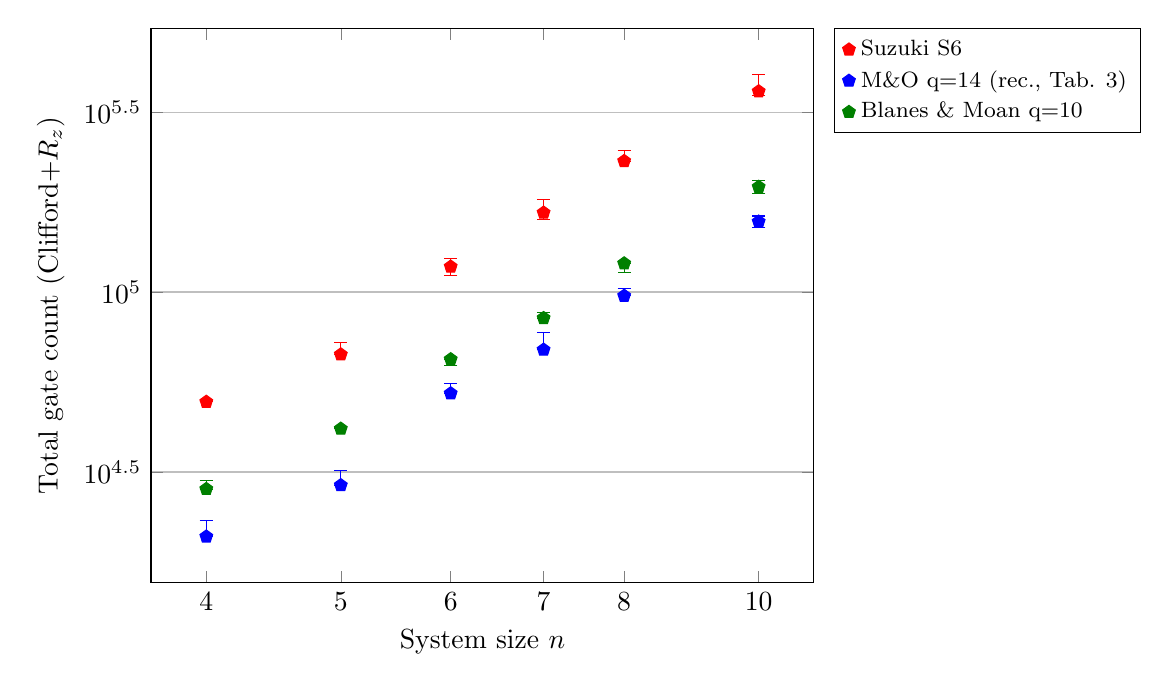
\begin{tikzpicture}
  \begin{loglogaxis}[
    width=10cm,
    xlabel={System size $n$},
    ylabel={Total gate count (Clifford+$R_z$)},
    xtick={4,5,6,7,8,10},
    xticklabels={4,5,6,7,8,10},
    ymajorgrids=true,
    legend pos=outer north east,
    legend cell align=left,
    legend style={font=\footnotesize},
  ]
    \addplot[only marks, red, mark=pentagon*, mark size=2.4pt, mark options={solid, fill=red}, error bars/.cd, y dir=both, y explicit, error bar style={red}] coordinates {
      (4,49536) += (0,0) -= (0,0)
      (5,67080) += (0,5160) -= (0,0)
      (6,117648) += (0,6192) -= (0,6192)
      (7,166152) += (0,14448) -= (0,7224)
      (8,231168) += (0,16512) -= (0,0)
      (10,361200) += (0,41280) -= (0,10320)
    };
    \addlegendentry{Suzuki S6}
    \addplot[only marks, blue, mark=pentagon*, mark size=2.4pt, mark options={solid, fill=blue}, error bars/.cd, y dir=both, y explicit, error bar style={blue}] coordinates {
      (4,20916) += (0,2324) -= (0,0)
      (5,29050) += (0,2905) -= (0,0)
      (6,52290) += (0,3486) -= (0,0)
      (7,69139) += (0,8134) -= (0,0)
      (8,97608) += (0,4648) -= (0,0)
      (10,156870) += (0,5810) -= (0,5810)
    };
    \addlegendentry{M\&O q=14 (rec., Tab. 3)}
    \addplot[only marks, green!50!black, mark=pentagon*, mark size=2.4pt, mark options={solid, fill=green!50!black}, error bars/.cd, y dir=both, y explicit, error bar style={green!50!black}] coordinates {
      (4,28356) += (0,1668) -= (0,0)
      (5,41700) += (0,0) -= (0,0)
      (6,65052) += (0,0) -= (0,2502)
      (7,84651) += (0,2919) -= (0,0)
      (8,120096) += (0,0) -= (0,6672)
      (10,195990) += (0,8340) -= (0,8340)
    };
    \addlegendentry{Blanes \& Moan q=10}
  \end{loglogaxis}
\end{tikzpicture}
